%% This is file `elsarticle-template-1-num.tex',
%%
%% Copyright 2009 Elsevier Ltd
%%
%% This file is part of the 'Elsarticle Bundle'.
%% ---------------------------------------------
%%
%% It may be distributed under the conditions of the LaTeX Project Public
%% License, either version 1.2 of this license or (at your option) any
%% later version.  The latest version of this license is in
%%    http://www.latex-project.org/lppl.txt
%% and version 1.2 or later is part of all distributions of LaTeX
%% version 1999/12/01 or later.
%%
%% Template article for Elsevier's document class `elsarticle'
%% with numbered style bibliographic references
%%
%% $Id: elsarticle-template-1-num.tex 149 2009-10-08 05:01:15Z rishi $
%% $URL: http://lenova.river-valley.com/svn/elsbst/trunk/elsarticle-template-1-num.tex $
%%
\documentclass[preprint,12pt]{elsarticle}

%% Use the option review to obtain double line spacing
%% \documentclass[preprint,review,12pt]{elsarticle}

%% Use the options 1p,twocolumn; 3p; 3p,twocolumn; 5p; or 5p,twocolumn
%% for a journal layout:
%% \documentclass[final,1p,times]{elsarticle}
%% \documentclass[final,1p,times,twocolumn]{elsarticle}
%% \documentclass[final,3p,times]{elsarticle}
%% \documentclass[final,3p,times,twocolumn]{elsarticle}
%% \documentclass[final,5p,times]{elsarticle}
%% \documentclass[final,5p,times,twocolumn]{elsarticle}

%% The graphicx package provides the includegraphics command.
\usepackage{graphicx}
%% The amssymb package provides various useful mathematical symbols
\usepackage{amssymb}
%% The amsthm package provides extended theorem environments
%% \usepackage{amsthm}
\usepackage{tabularx}
%% The lineno packages adds line numbers. Start line numbering with
%% \begin{linenumbers}, end it with \end{linenumbers}. Or switch it on
%% for the whole article with \linenumbers after \end{frontmatter}.
\usepackage{lineno}
\usepackage[round]{natbib}
%% natbib.sty is loaded by default. However, natbib options can be
%% provided with \biboptions{...} command. Following options are
%% valid:

%%   round  -  round parentheses are used (default)
%%   square -  square brackets are used   [option]
%%   curly  -  curly braces are used      {option}
%%   angle  -  angle brackets are used    <option>
%%   semicolon  -  multiple citations separated by semi-colon
%%   colon  - same as semicolon, an earlier confusion
%%   comma  -  separated by comma
%%   numbers-  selects numerical citations
%%   super  -  numerical citations as superscripts
%%   sort   -  sorts multiple citations according to order in ref. list
%%   sort&compress   -  like sort, but also compresses numerical citations
%%   compress - compresses without sorting
%%
%% \biboptions{comma,round}

% \biboptions{}

\journal{Hydrological Procesesses}

\begin{document}

\begin{frontmatter}

%% Title, authors and addresses

\title{Surface and subsurface runoff hydrological partitioning. The role of rainfall features and antecedent soil moisture conditions in a tropical watershed.}

%% use the tnoteref command within \title for footnotes;
%% use the tnotetext command for the associated footnote;
%% use the fnref command within \author or \address for footnotes;
%% use the fntext command for the associated footnote;
%% use the corref command within \author for corresponding author footnotes;
%% use the cortext command for the associated footnote;
%% use the ead command for the email address,
%% and the form \ead[url] for the home page:
%%
%% \title{Title\tnoteref{label1}}
%% \tnotetext[label1]{}
%% \author{Name\corref{cor1}\fnref{label2}}
%% \ead{email address}
%% \ead[url]{home page}
%% \fntext[label2]{}
%% \cortext[cor1]{}
%% \address{Address\fnref{label3}}
%% \fntext[label3]{}


%% use optional labels to link authors explicitly to addresses:
%% \author[label1,label2]{<author name>}
%% \address[label1]{<address>}
%% \address[label2]{<address>}

\author[1,2]{N. Velasquez}
\author[2]{S. Castillo}
\author[2, 3]{C.D. Hoyos}

\address[1]{Iowa University, IIHR}
\address[2]{EAFIT university.}
\address[3]{Universidad nacional de Colombia.}

\begin{abstract}
%% Text of abstract
Suspendisse potenti. Suspendisse quis sem elit, et mattis nisl. Phasellus consequat erat eu velit rhoncus non pharetra neque auctor. Phasellus eu lacus quam. Ut ipsum dolor, euismod aliquam congue sed, lobortis et orci. Mauris eget velit id arcu ultricies auctor in eget dolor. Pellentesque suscipit adipiscing sem, imperdiet laoreet dolor elementum ut. Mauris condimentum est sed velit lacinia placerat. Vestibulum ante ipsum primis in faucibus orci luctus et ultrices posuere cubilia Curae; Nullam diam metus, pharetra vitae euismod sed, placerat ultrices eros. Aliquam tincidunt dapibus venenatis. In interdum tellus nec justo accumsan aliquam. Nulla sit amet massa augue.
\end{abstract}

\begin{keyword}
Science \sep Publication \sep Complicated
%% keywords here, in the form: keyword \sep keyword

%% MSC codes here, in the form: \MSC code \sep code
%% or \MSC[2008] code \sep code (2000 is the default)

\end{keyword}

\end{frontmatter}

%%
%% Start line numbering here if you want
%%
\linenumbers

%#################################################################
%% main text
\section{Introduction}
\label{intro}

During a storm event the hydrograph is mainly formed by surface and subsurface runoff volumes \citep{Flury1994,Jackisch2016}. The separation of those runoff volumes is referred to as flow partitioning \citep{Munoz2012}. Soils, land use, topography, and external forcings such as rainfall spatio-temporal patterns, and pre-event water, modulate the surface and subsurface partition \citep{radatz2013, Shope2016}. Understanding the link between flow partitioning and external forcings is fundamental for catchment hydrology assessment and hydrological model implementation \citep{todd2006,Tetzlaff2008}.  Due to this relevance, several methods have been used to assess the characterization of flow partitioning, including field techniques \citep{Shope2016}, tracers \citep{Tetzlaff2008}, digital filters \citep{Eckhardt2005,Stewart2015a}, and modeling approximations \citep{Partington2011, Dukic2006}.  In spite of the several attempts, the large number of techniques, and the differences in the results, there is no consensus on which is the best approach to analyze forcings on runoff mechanisms during storm events (\citep{Stewart2015a, Blume2015, Penna2015}. The  high level of subjectivity still involved in such analysis indicates that the problem is not fully understood \citep{Dukic2006, Tallaksen1995}.\\

Despite the above mentioned differences, it is clear that subsurface runoff plays a crucial role during storm events \citep{Pinder1969, Sklash1979, Wels1991, Zehe2010,Blume2015, Jackisch2016}.  Evidence could be found in several cases. Using tracers in three basins of Nova Scotia, \citet{Pinder1969} found that around 40\% of the total runoff is explained by subsurface.  \citet{Eckhardt2005} obtains a similar result using digital filters,  with subsurface contribution oscillating between 25 and 80\% of the streamflow.  \citet{Shope2016} presented a similar result in the Haean-Myun catchment (South-Korea), with subsurface contributions around 46\% of the hydrograph.  There are also indirect results that reinforce the idea of a strong subsurface flow participation. Using field observations and simulations,  \citet{Sklash1979} found large and rapid increases of the hydraulic head in the near-stream groundwater after the start of the rain. \citet{Kubota1995} compared modeled results with observations, and showed that a significant portion of the streamflow is explained by subsurface runoff equations.\\ 

Subsurface stormflow portion tends to be highly variable, characteristic that rises questions regarding the processes and the interaction with forcing variables such as rainfall or pre-event water \citep{Dunkerley2017, Jackisch2016, Torch2013}.  Rainfall external forcing exhibits a high spatiotemporal variability which may impact the hydrograph partitioning.  High intense events, with low accumulation and short duration, increase surface and lower subsurface production CITA(Liu, 2016).  On the other hand, low intensity and long duration rainfall events, increase subsurface volume \citep{Rusjan2015, Blume2015}. By inducing synthetic abrupt temporal variations in the rainfall, \citep{Dunkerley2008} found significant reductions of the runoff production. The rainfall interactions variability are not limited to high or low intensities, they change also in function of the basin area, topography and soil textures \citep{Shope2016, Shope2014}. According to \citep{Mei2015a} rainfall duration increases with the basin area, and so does the subsurface production.  Also, field findings suggest rainfall features and their variability influence partitioning and the displacement of pre-event water \citep{Zabaleta2013, Penna2011}.  The mentioned results give an idea about the role of the rainfall.  However, there is a lack of evidence that links rainfall spatio-temporal variability with the dynamic of the stormflow partitioning \cite{Gomi2010}.\\

In addition to rainfall, pre-event water also plays a crucial role on the stormflow partitioning variability \citep{Dusek2016, Klaus2013,Clow2000,Sklash1979}. Although subsurface runoff could be different from pre-event water, both variables are highly correlated \citep{Wels1991, Rusjan2015}. Using isotopes, \citet{Sklash1979} showed that pre-event water dominated the hydrograph in humid systems.  In another humid watershed, \citet{Cey1998} found that pre-event water explains the 80\% of the hydrograph.  A comparable value was reported by \citet{Buda2009} for a 45$km^2$ catchment.  Bazemore (1994) observed that pre-event water increases contribution to the transient saturated zone during storm events.  In a small catchment, \citet{Dewalle1994} reported a pre-event water participation between 55 and 94\%.  Similar values were reported by \citet{Carey2005} with pre-event water ratios above 50\%. In a small catchment (0.198$km^2$). \citet{Munyaneza2012} reported pre-event water contributions of 60 and 80\% for catchments with areas of 129 and 257.4$km^2$ respectively.  Additionally, the participation and influence of pre-event water on the hydrograph partitioning could be partially conditioned by the rainfall variability \citet{Clow2000}.\\  

In the present work, we want to explore how the variability of both forcings (rainfall and pre-event water) and their interplay influence stormflow partitioning. Using a modeling approach, we analyze rainfall and pre-event water interactions on the hydrograph partitioning in a tropical catchment. We use the distributed hydrological model WMF (Watershed Modeling Framework) \citep{Frances2007}, with the ability to separate surface and subsurface runoff.  Rainfall is derived from a C-band weather radar, model calibration and validation is achieved with a stage station data located at basin outlet. Pre-event water is analyzed from model states obtained with an hourly scale simulation achieved for reccords between 2013-2017. Then, stormflow partition is analyzed for each event simulated at a 5min time step for each event, simulations at 5 min. scale is carried out and stormflow partition is analyzed for each event using at a 5 min time step simulation. Variability of simple features such as maximum intensity and total stored volume are contrasted against the flow partitioning. The experiment was conducted with 128 storm events to get conclusive results about the catchment response under storm events.\\

%#################################################################
%% main text
\section{Data and methods}
\label{methods}
We present the overall methodology followed in the present work in an illustrative diagram in Figure 2.  For the experiment, we made a mid-term simulation with the distributed hydrological model at a time step of one hour for the period between 2013 and 2017.  In this same period, we did simulate 128 storm events with the conditions obtained from the mid-term simulation.  For each event, the model separates surface and subsurface runoff, which was then compared against rainfall and pre-event water features. The rainfall features include intensity, depth, and days since the last storm.  On the other hand, soil conditions features include the mean gravitational storage from three hours before each storm event, and the time passed since the last storm event.\\

\subsection{Study and area}

The current work is done in the Valle de Aburrá (VA) watershed, located on the north-east part of Central Colombian Andes (see Figure \ref{fig:localization}).  In the region, there is a high frequency of local convective cores which produce intense storm events \citep{Zuluaga2015}. This fact along with locally steep slopes and the urbanization of the watershed (24\% of the total area), produces abrupt changes in the streamflow during storm events. Also, there are human settlements near steep network tributaries subject to abrupt changes.  The mentioned characteristics give hydrological and political relevance to the analysis of the hydrograph formation during storm events. 

Several information resources were used to develop the analysis.  ALOS-PALSAR elevation raster data \citep{ALOS} was used for the basin delineation and also for the estimation of the distributed geomorphological parameters.  From POMCA (a local environmental project of the watershed) we obtained land use, roughness and soil information. Soils hydraulic properties were derived from the soils texture descriptions by using the SPAW software \citep{Saxton2006}.

\begin{figure}[t]
    \centering
    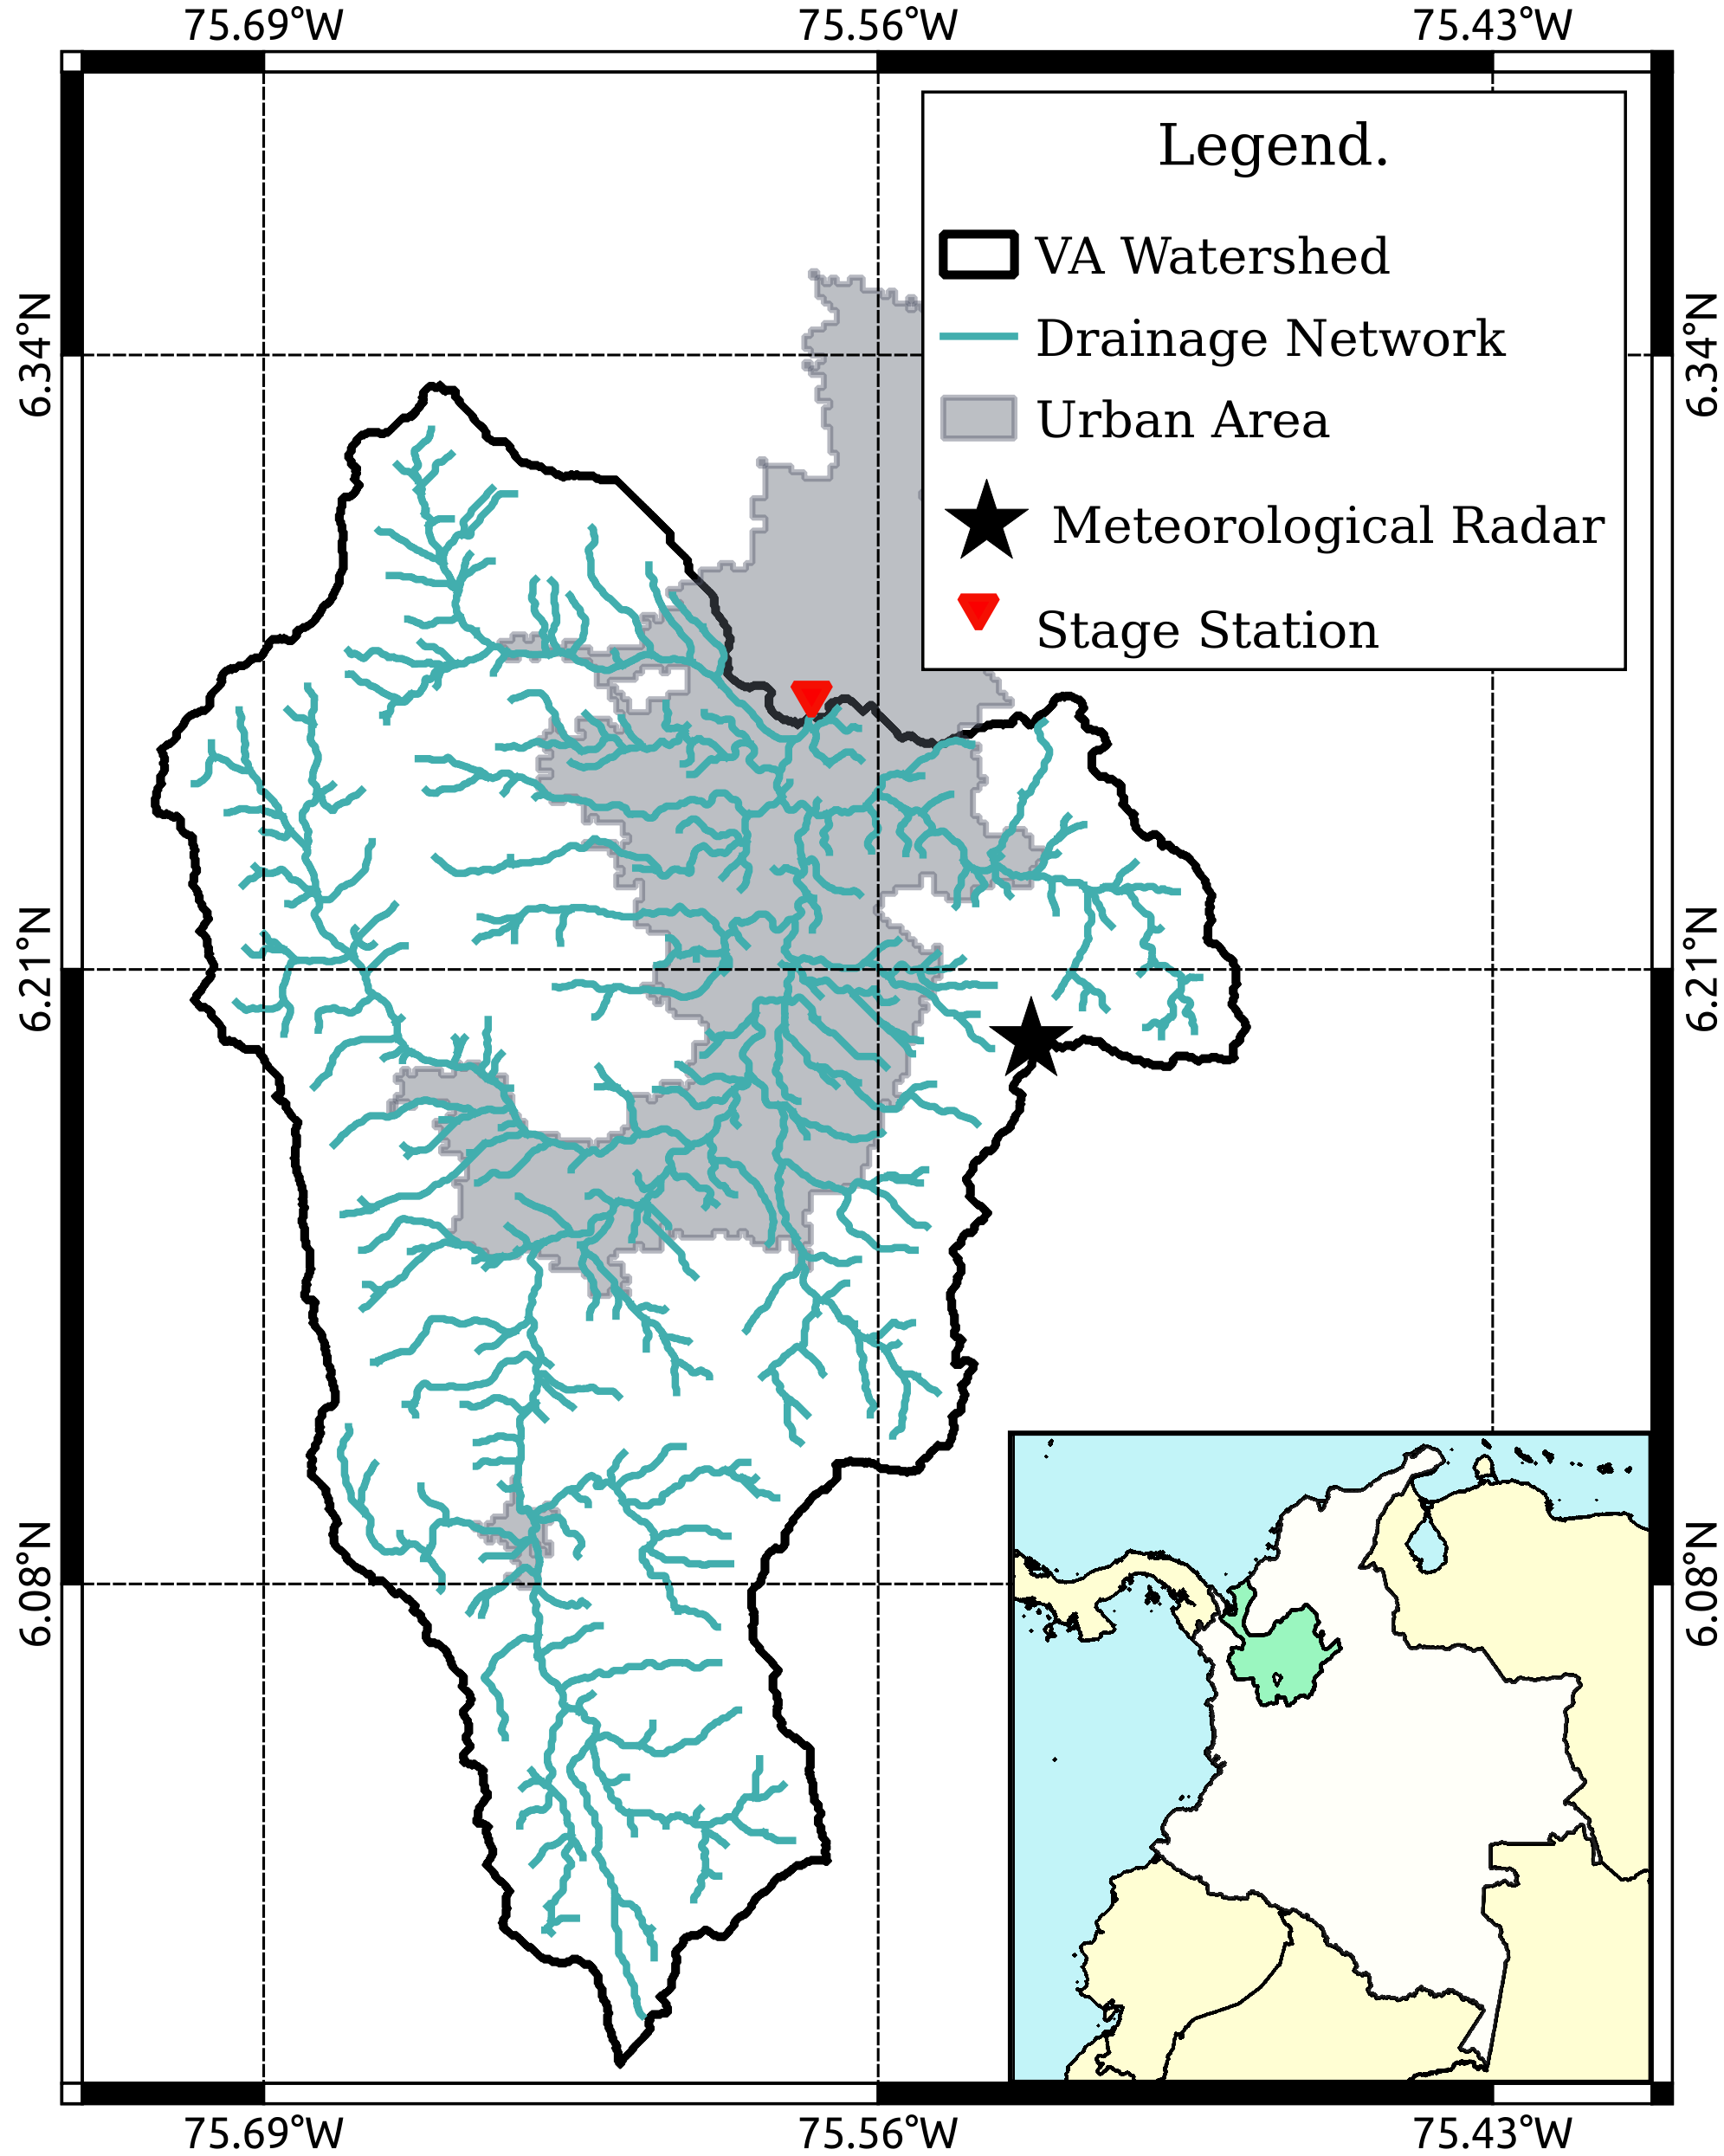
\includegraphics[width=8.3cm]{Figuras/layout_aula3.png}
    \caption{Watershed, radar and stream gauge localization.}
    \label{fig:localization}
\end{figure}

VA is a typical tropical mountainous basin with variable topographical and soil textures. The main channel presents a mean slope of 1.83\%, it starts at approximately 2300 masl, while the outlet is around 1400 masl (884 m of height gradient). In contrast, some sub-basins show height differences of 2000$m$. The mean basin slope is about 30\%, with some hills reaching values between 50\% and 80\%.  Soils are mainly composed of sand and silt with a low percentage of clay (POMCA, 2007). Depths estimations of the soil profile (Z) oscillate between 0.2 and 1 m \citep{Osorio2008}, being deeper at the foothills than at the slopes development. Hydraulic conductivity (Ks) varies between 10 and 125 mm/h, with higher values on the hills in the south-west.  The hydraulic properties of the soils led to the estimation of the capillary ($H_u$) and gravitational ($H_g$) storage capacity. $H_u$ oscillates between 20 and 200 $mm$ and $H_g$ between 15 and 500$mm$.\\

Used temporal information includes a local level station located at the outlet of the basin (red triangle at Figure \ref{fig:localization}) and QPE estimations from a meteorological radar.  The level information dates from 2011 to 2018 with a time step of 1min.  The QPE technique was developed by Sepúlveda and Hoyos (2018).  This technique uses retrievals from a C-band polarimetric Doppler weather radar operated by the Sistema de Alertas Tempranas de Medellín y del Valle de Aburra (SIATA).  The quality of the radar data is high due to its vicinity to the basin (black star at Figure \ref{fig:localization}), however, the radar does not detect information in its immediate vicinity (blue circle in Figure \ref{fig:localizacion}).  Due to the operating strategy of the radar the information is collected every 5$min$ at a spatial resolution of 128 $m$.\\

Temporal information consists of a stage station located at the basin outlet and the mentioned QPE estimations; both records were obtained by the local early warning system (Sistema de Alerta Temprana de Medellín y el Valle de Aburrá, SIATA). The stage station is over the main channel; it counts with several streamflow measurements which lead to a robust rating curve.\\

\subsection{Hydrological model and flow separation }

For the hydrological simulation, we use a modification of the distributed hydrological model proposed by \citep{Frances2007, Velez2001}.  The model discretizes the watershed into cells, for this case we use a resolution of 30x30m.   In each cell, five tanks represent the hydrological storages: capillary (tank 1), gravitational (tank 2), runoff (tank 3), baseflow (tank 4) and streamflow  (tank 5).  The state of each tank ($S_i$) varies in function of the vertical and lateral flows as shown in Figure 2,  $S_i$ varies in function of its inputs ($D_i$) and outputs ($E_i$). The value of $D_i$ oscillates in function of the vertical inflow ($R_i$) and the vertical interaction with its surrounding tanks.  For tank 1, the input is represented by the rainfall at the cell ($R_1$) and the output $E_1$ corresponds to the evaporated water, in the remaining tanks $E_i$ corresponds to a horizontal outflow. 

Based on two threshold accumulated areas, the model classifies the watershed into three types of cells: hill cells, cells with ephemeral streams, and cells with perennial streams.  The connection between tanks and cells varies in relation to the types of cells.  At hill cells, $E_i$ goes to the same tank of the downstream cell.  At ephemeral cells,$E_2$ and $E_3$ go to tank 5 and $E_4$ goes to the cell downstream. In the perennial cells, $E_2$, $E_3$ and $E_4$ go to tank 5.  $E_5$ goes downstream for both ephemeral and perennial streams.  At tanks 2, 3 and 5 the lateral flow $E_i$ is approximated by a kinematic equation.  Surface runoff speed ($E_2$) is explained by a modification of Manning's formula for flow in gullies \citep{Foster1984} (equation \ref{eq:foster}).  Subsurface runoff ($E_3$) is explained by the \citep{Kubota1995} approximation (equation \ref{eq:kubota}).  The subterranean flow ($E_4$) is assumed as a linear tank. And, the Geomorphologic Kinematic Wave approximation \citep{Velez2001} is used to estimate the channel flow ($E_5$) speed.  More information on the model could be found at \citep{Velez2001, Frances2007}. \\

\begin{equation}
 v_{2} = \frac{\varepsilon}{n}  S_{0}^{1/2} A_{2}(t)^{(2/3) e_1}
    \label{eq:foster}
\end{equation}

\begin{equation}
 v_3 = \frac{K_s S_{o}^{2}}{(b+1) A_{g}^{b}} A_{3}(t)^{b}
    \label{eq:kubota}
\end{equation}

\begin{equation}
 v_4 = \Omega A_4^{\omega_1} S_0^{\omega_2} \Lambda^{\omega_3} 
    \label{eq:ocg}
\end{equation}

In addition to the hydrological processes, the model can track surface (tank 2) and subsurface (tank 3) streamflow contribution at each channel reach. It marks water once it reaches any of those two tanks, and the surface-subsurface flow percentage is taken into account once the water enters tank 5 (the channel).   At this point, the model assumes that the water in the channel is well mixed,  implying that the surface and subsurface portions are constant until a new inflow enters the channel.  It is important to notice that this estimation does not interfere with the calculation of the flow process downstream.\\ 

\subsection{Experiment set}

We parametrize and validate the model for a mid-term simulation with an hourly time step, and also at event-scale (5min).  For this, we used the radar and streamflow registers between 2013 and 2017.  At each time step, we saved the states of the mid-term model which were then used as the initial conditions for the event simulations.  The streamflow partitioning only works over the events simulated at 5min scale.\\

The primary goal of the present work is to analyze how rainfall and pre-event soil water influence surface and subsurface partitioning during storm events.  With this regard, we perform a qualitative evaluation of four selected events and a quantitative analysis including all the cases (128).  The qualitative analysis considers the spatiotemporal variations of the observed rainfall, the simulated and observed streamflows ($Q_{obs}$ and $Q_{sim}$ respectively), an the model partitioned surface and subsurface streamflows ($Q_{run}$ and $Q_{sub}$ respectively).  For the quantitative analysis, we analyze two main features of the rainfall: the maximum mean intensity ($I_{max}$), and the total rainfall depth ($P_{tot}$).  $I_{max}$ is obtained directly from the rainfall hietogram, which is obtained at each time step $t$ as the mean intensity observed by the radar, and $P_{tot}$ is the sum of the hietogram at the end of the event.  We also consider the model soil storage ($S_3$), and the dry hours before each event ($T_{dry}$) as proxies of the pre-event soil water for each event.   Finally, we compared the mentioned variables against the hydrograph volume partitioned by the model as $V_{sur}$ (surface runoff volume) and $V_{sub}$ (subsurface runoff volume).\\

%#################################################################
%% main text
\section{Results and Analysis}
\label{results}

The model performance was evaluated at a mid-term scale (hourly) and at an event scale (5min) for each one of the N events.  There is an overall good performance of the model in the mid-term simulation (NE value of XX and Figure 4), which gave us confidence about the initial conditions for the event scale simulations. In the event scale, the model starts the simulation 3 hours before the peak-flow and ends 3 hours after.  For a more comprehensive analysis, four events were analyzed in detail, considering spatiotemporal variations of the rainfall by a qualitative analysis of the radar fields.  Complementary, we analyzed streamflow partitioning variability of all events involving the total partitioned volume, rainfall features, and pre-event conditions.  Results show that streamflow partitioning depends on pre-event water, rainfall variability, and their interplay.\\      

\subsection{Parameterization and validation}

In the parametrization process, we search for scalar values corresponding to each physical variable of the model \citep{Frances2007}.  The search ends when the model simulated streamflow fits the observed streamflow at the outlet (red station at Figure \ref{fig:localization}).  At Table \ref{tab:parameters} we show the obtained parameters for the hourly and 5min simulations.  At both scales, the values of $H_u$ and $H_g$ are equal. Moreover, the most sensitive parameters correspond to the subsurface hydraulic conductivity ($K_s$), deep conductivity ($K_p$), surface flow velocity ($V_1$) and subsurface flow velocity ($V_2$).\\

\begin{table}[]
        \centering
        \begin{tabularx}{\textwidth}{p{3cm} p{2.2cm} p{1.5cm} p{2cm} p{3.5cm}}
\hline
Parameter Name & Symbol & Long term & Event & Spatial distribution \\
\hline
Capilary storge & Hu [mm] & 1 & 39 & In function of the slope \\
Gravitational storage & Hg [mm] & 1 & 34 & As a function of the slope \\
Evaporation rate & Etr [mm/s] & 0.1 & 0.01 & As a function of the DEM \\
Infiltration rate & ks [mm/s] & 2.7 & 0.0012 & Lumped \\
Percolation rate & kp [mm/s] & 0.8 & 0.00012 & Lumped \\
System losess & Kf [mm/s] & 0 & 0.0 & Lumped \\
Surface speed & vr [m/s] & 0.5 & 6.4 & As a function of the slope and storage \\
Subsurface speed & vs [m/s] & 1 & 7.1 & As a function of the slope, Hg and storage\\
Subterranean speed & vb [m/s] & 0.5 & 0.000095 & Lumped \\
Channel speed & vc [m/s] & 1 & 0.95 & As a function of the slope, acumulated area, and storage \\
\hline
\end{tabularx}
        \caption{Hydrologic model parameters.}
        \label{tab:parameters}
    \end{table}

The results shows that the model has an overall acceptable performance.  At an hourly scale, the model achieves an $NE$ value of 0.3 which is an acceptable performance considering that it is out of the focus of the present work.  At the event scale, the performance considers $NE$, $QmaxDif$ (peak streamflow difference), and $VtotDif$ (total volume difference).  For 40\% of the events the model gets $NE$ values above 0.6, $50\%$ with $NE$ values above 0.4, and $QmaxDIf$ values below XX, a distribution of the event-scale performance is shown in Figure \ref{fig:performance}.  Considering that poor performance events could bias our analysis, we only consider events with $NE$ values above 0.4.\\

\begin{figure}[t]
    \centering
    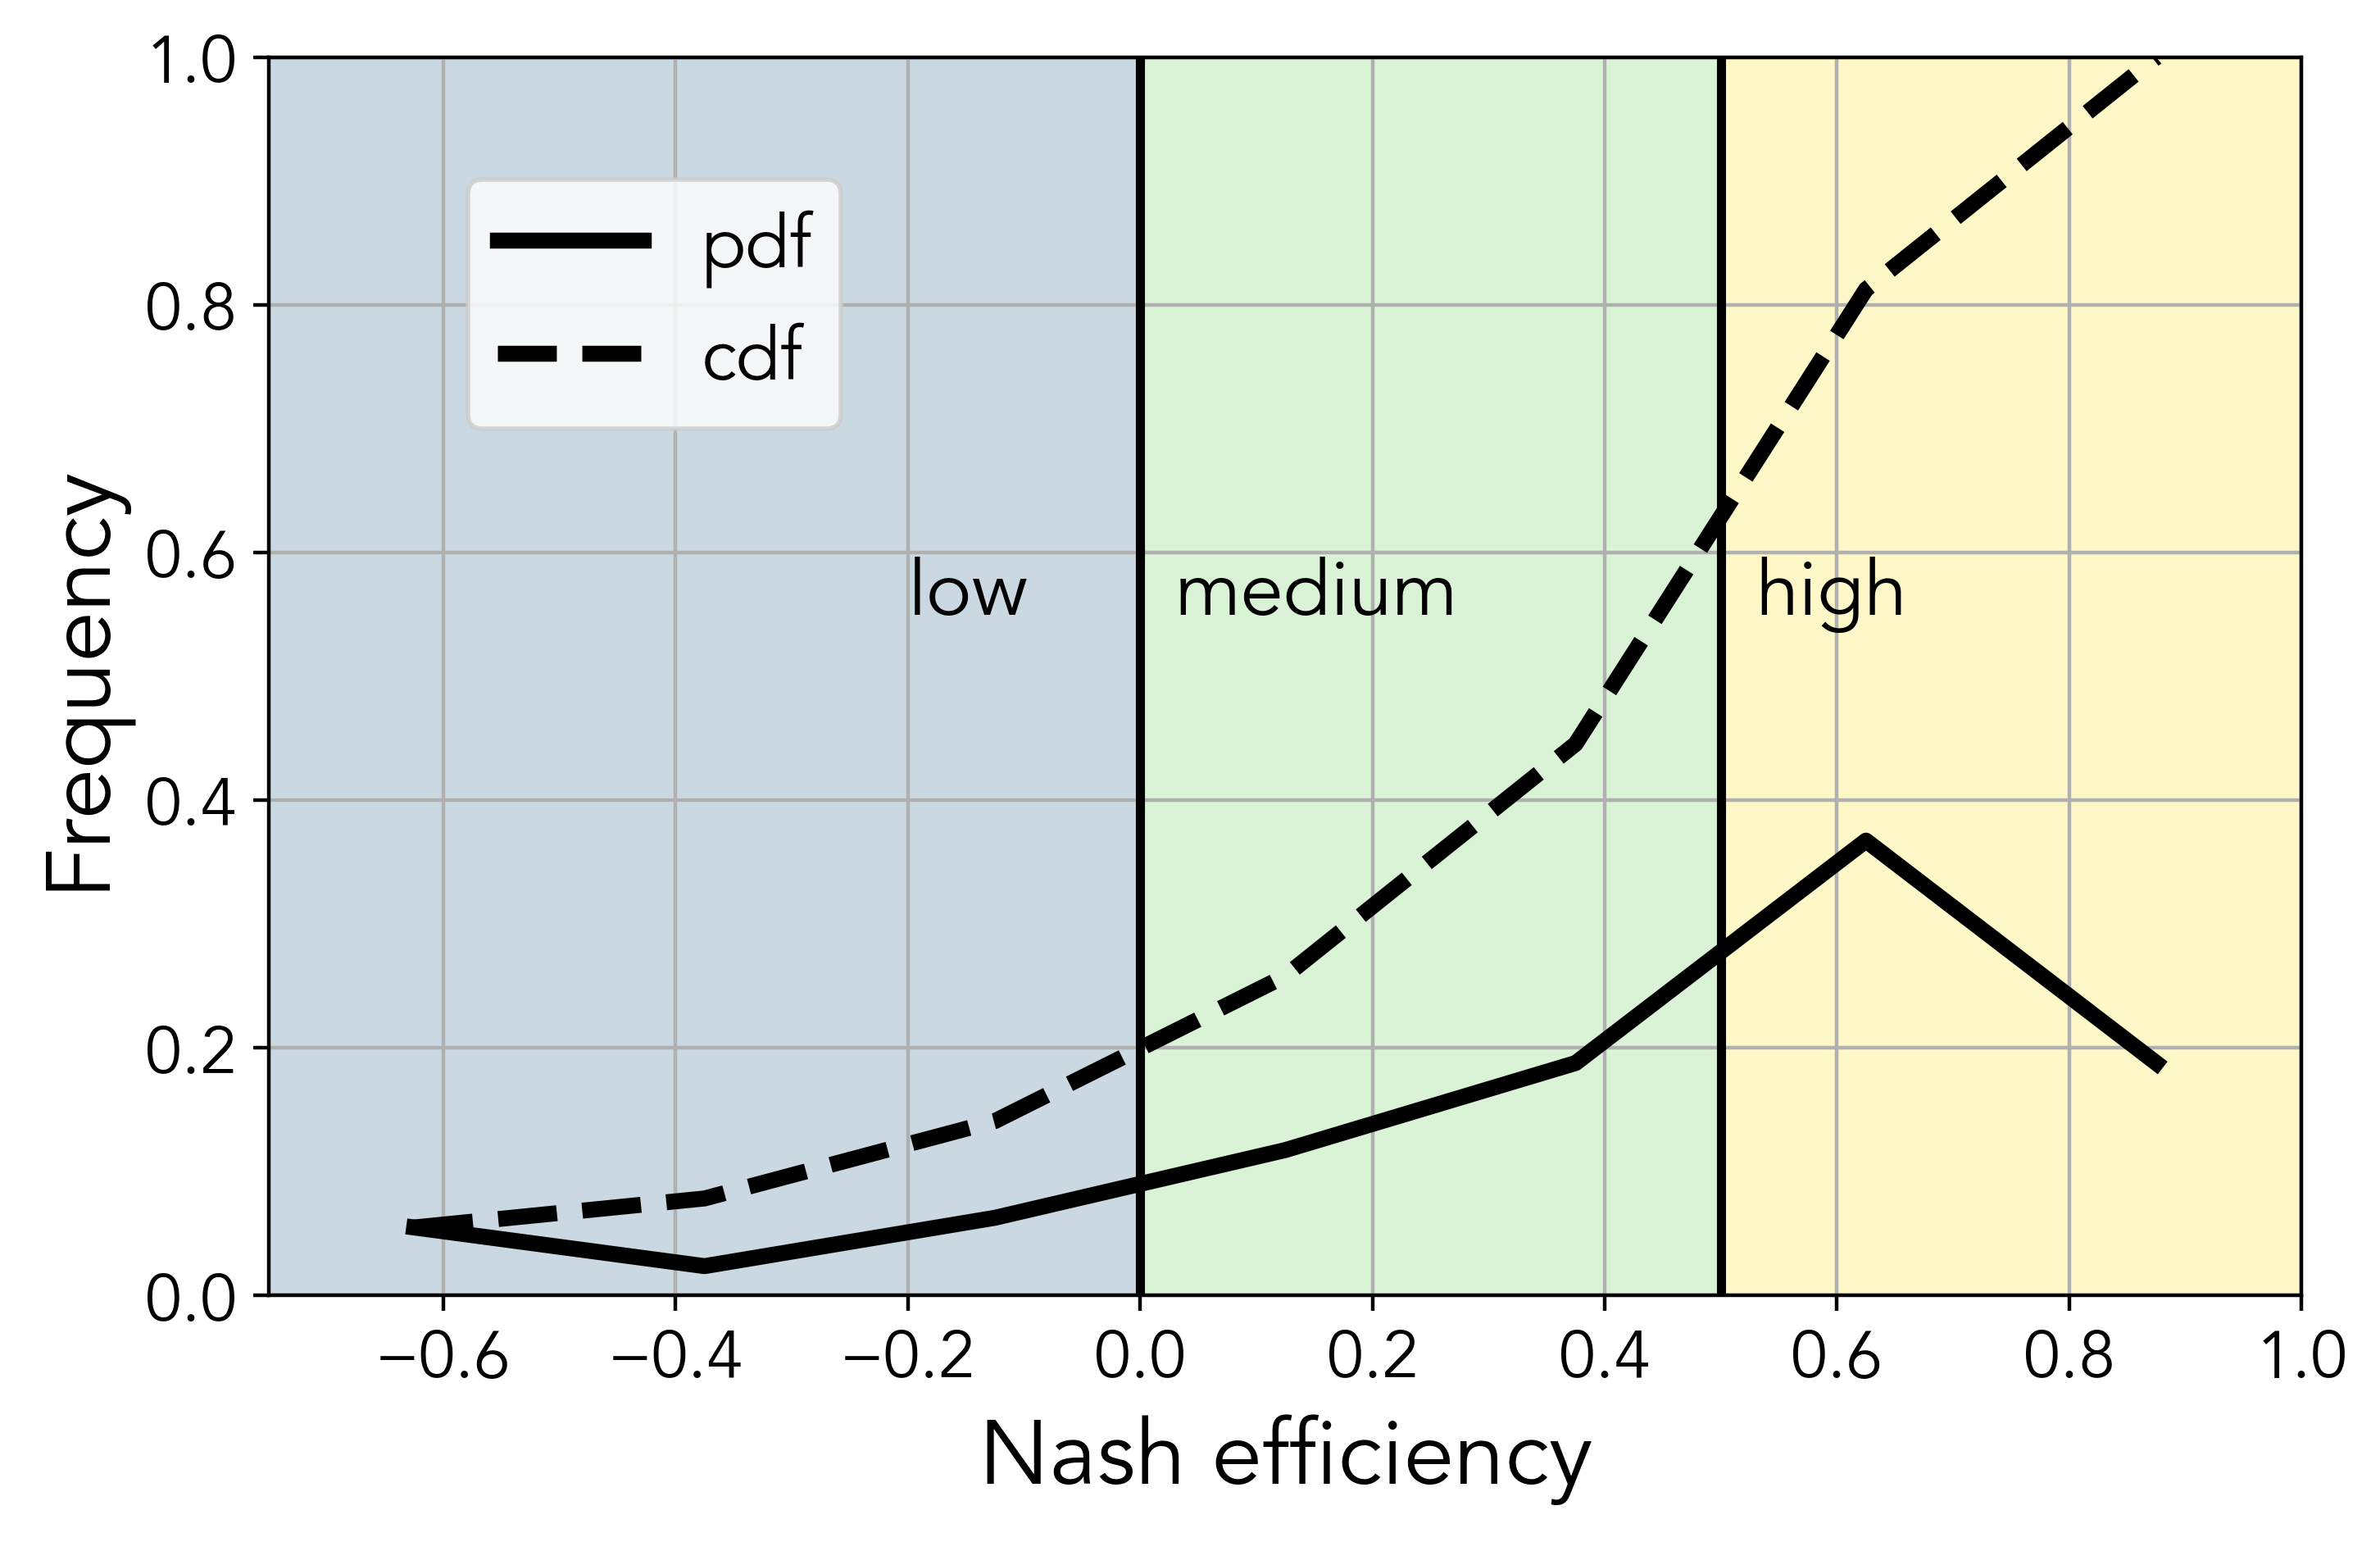
\includegraphics[width=8.3cm]{Figuras/PerformNS_pdf.png}
    \caption{Nash sutcliffe performance distribution for the analyzed events.}
    \label{fig:performance}
\end{figure}

\subsection{Stormflow partitioning at 4 specific cases } \label{sec:4Cases}

We first analyzed in detail 4 events in order to assess how variations at rainfall and soil moisture condition the streamflow partitioning. The four events were selected by their variations of the total percentage of surface and subsurface runoff.  According to this, there are two well mixed events, one surface dominated event, and a subsurface dominated one (Figure \ref{fig:four_events}). For the analysis, we took into account the hietogram evolution, rainfall spatial accumulation (Figure \ref{fig:rainfall_acum}), and radar profiles at different time steps (Figure \ref{fig:radar_profiles}).\\

At the end of each event, the spatial rainfall accumulation is different, however there are some similarities. We have two events with an homogeneous rainfall accumulation fields, and two events dominated by convective storm formations. The homogeneous events correspond to  E100 and E186 (Figures \ref{fig:rainfall_acum}a and d respectively) where spatial  rainfall accumulation reaches low to medium levels. On the other hand, event E120 (Figure \ref{fig:rainfall_acum}b) has one convective system of high rainfall accumulation in the middle of the watershed.  And E123 (Figure \ref{fig:rainfall_acum}c) shows different regions with important rainfall accumulations (convective cores).  Both, events E120 and E123 have high rainfall accumulations over the urban area of the watershed.\\

\begin{figure}[!h]
    \centering
    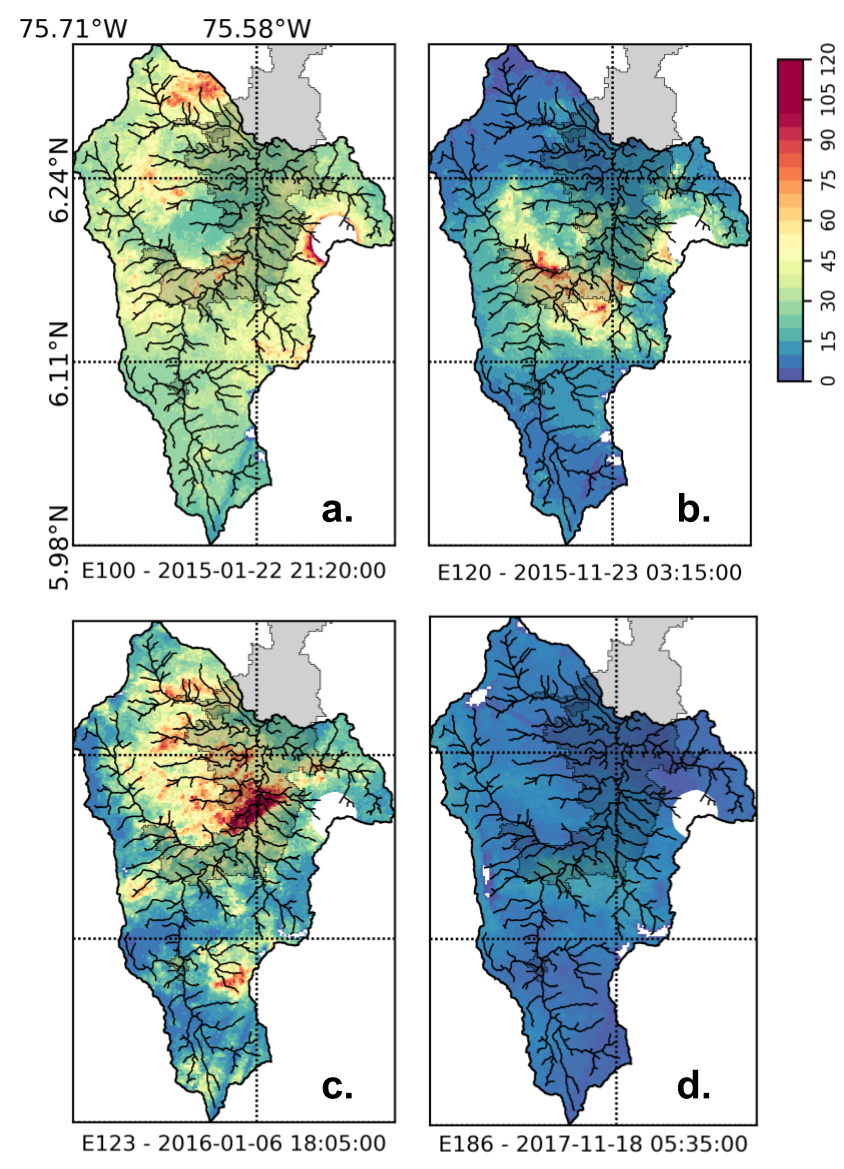
\includegraphics[width=14cm]{Figuras/Rainfall_accumulation.png}
    \caption{Total accumulated rainfall at the end of the event.  From panels a to d we show respectively events E100, E120, E123 and E186.}
    \label{fig:rainfall_acum}
\end{figure}
Complementary to the rainfall accumulation, at Figure \ref{fig:radar_profiles} we present the evolution of the storms observed as radar vertical profiles. In this evolution we can see additional differences among the events.  According to the profiles, E100 is an event of stratiform nature, with well defined layers and low rainfall accumulation.  On the other hand, E120 and E123 exhibit well defined convective formations.  In the case of E120 the convective cell appears at the beginning of the event, and eventually evolves as a stratiform storm.  On E123 the convective cell covers more area of the watershed, and has an important vertical development.  The evolution of the four rainfall events is also shown on the hietograms presented at Figure \ref{fig:four_events}.  

\begin{figure}[!h]
    \centering
    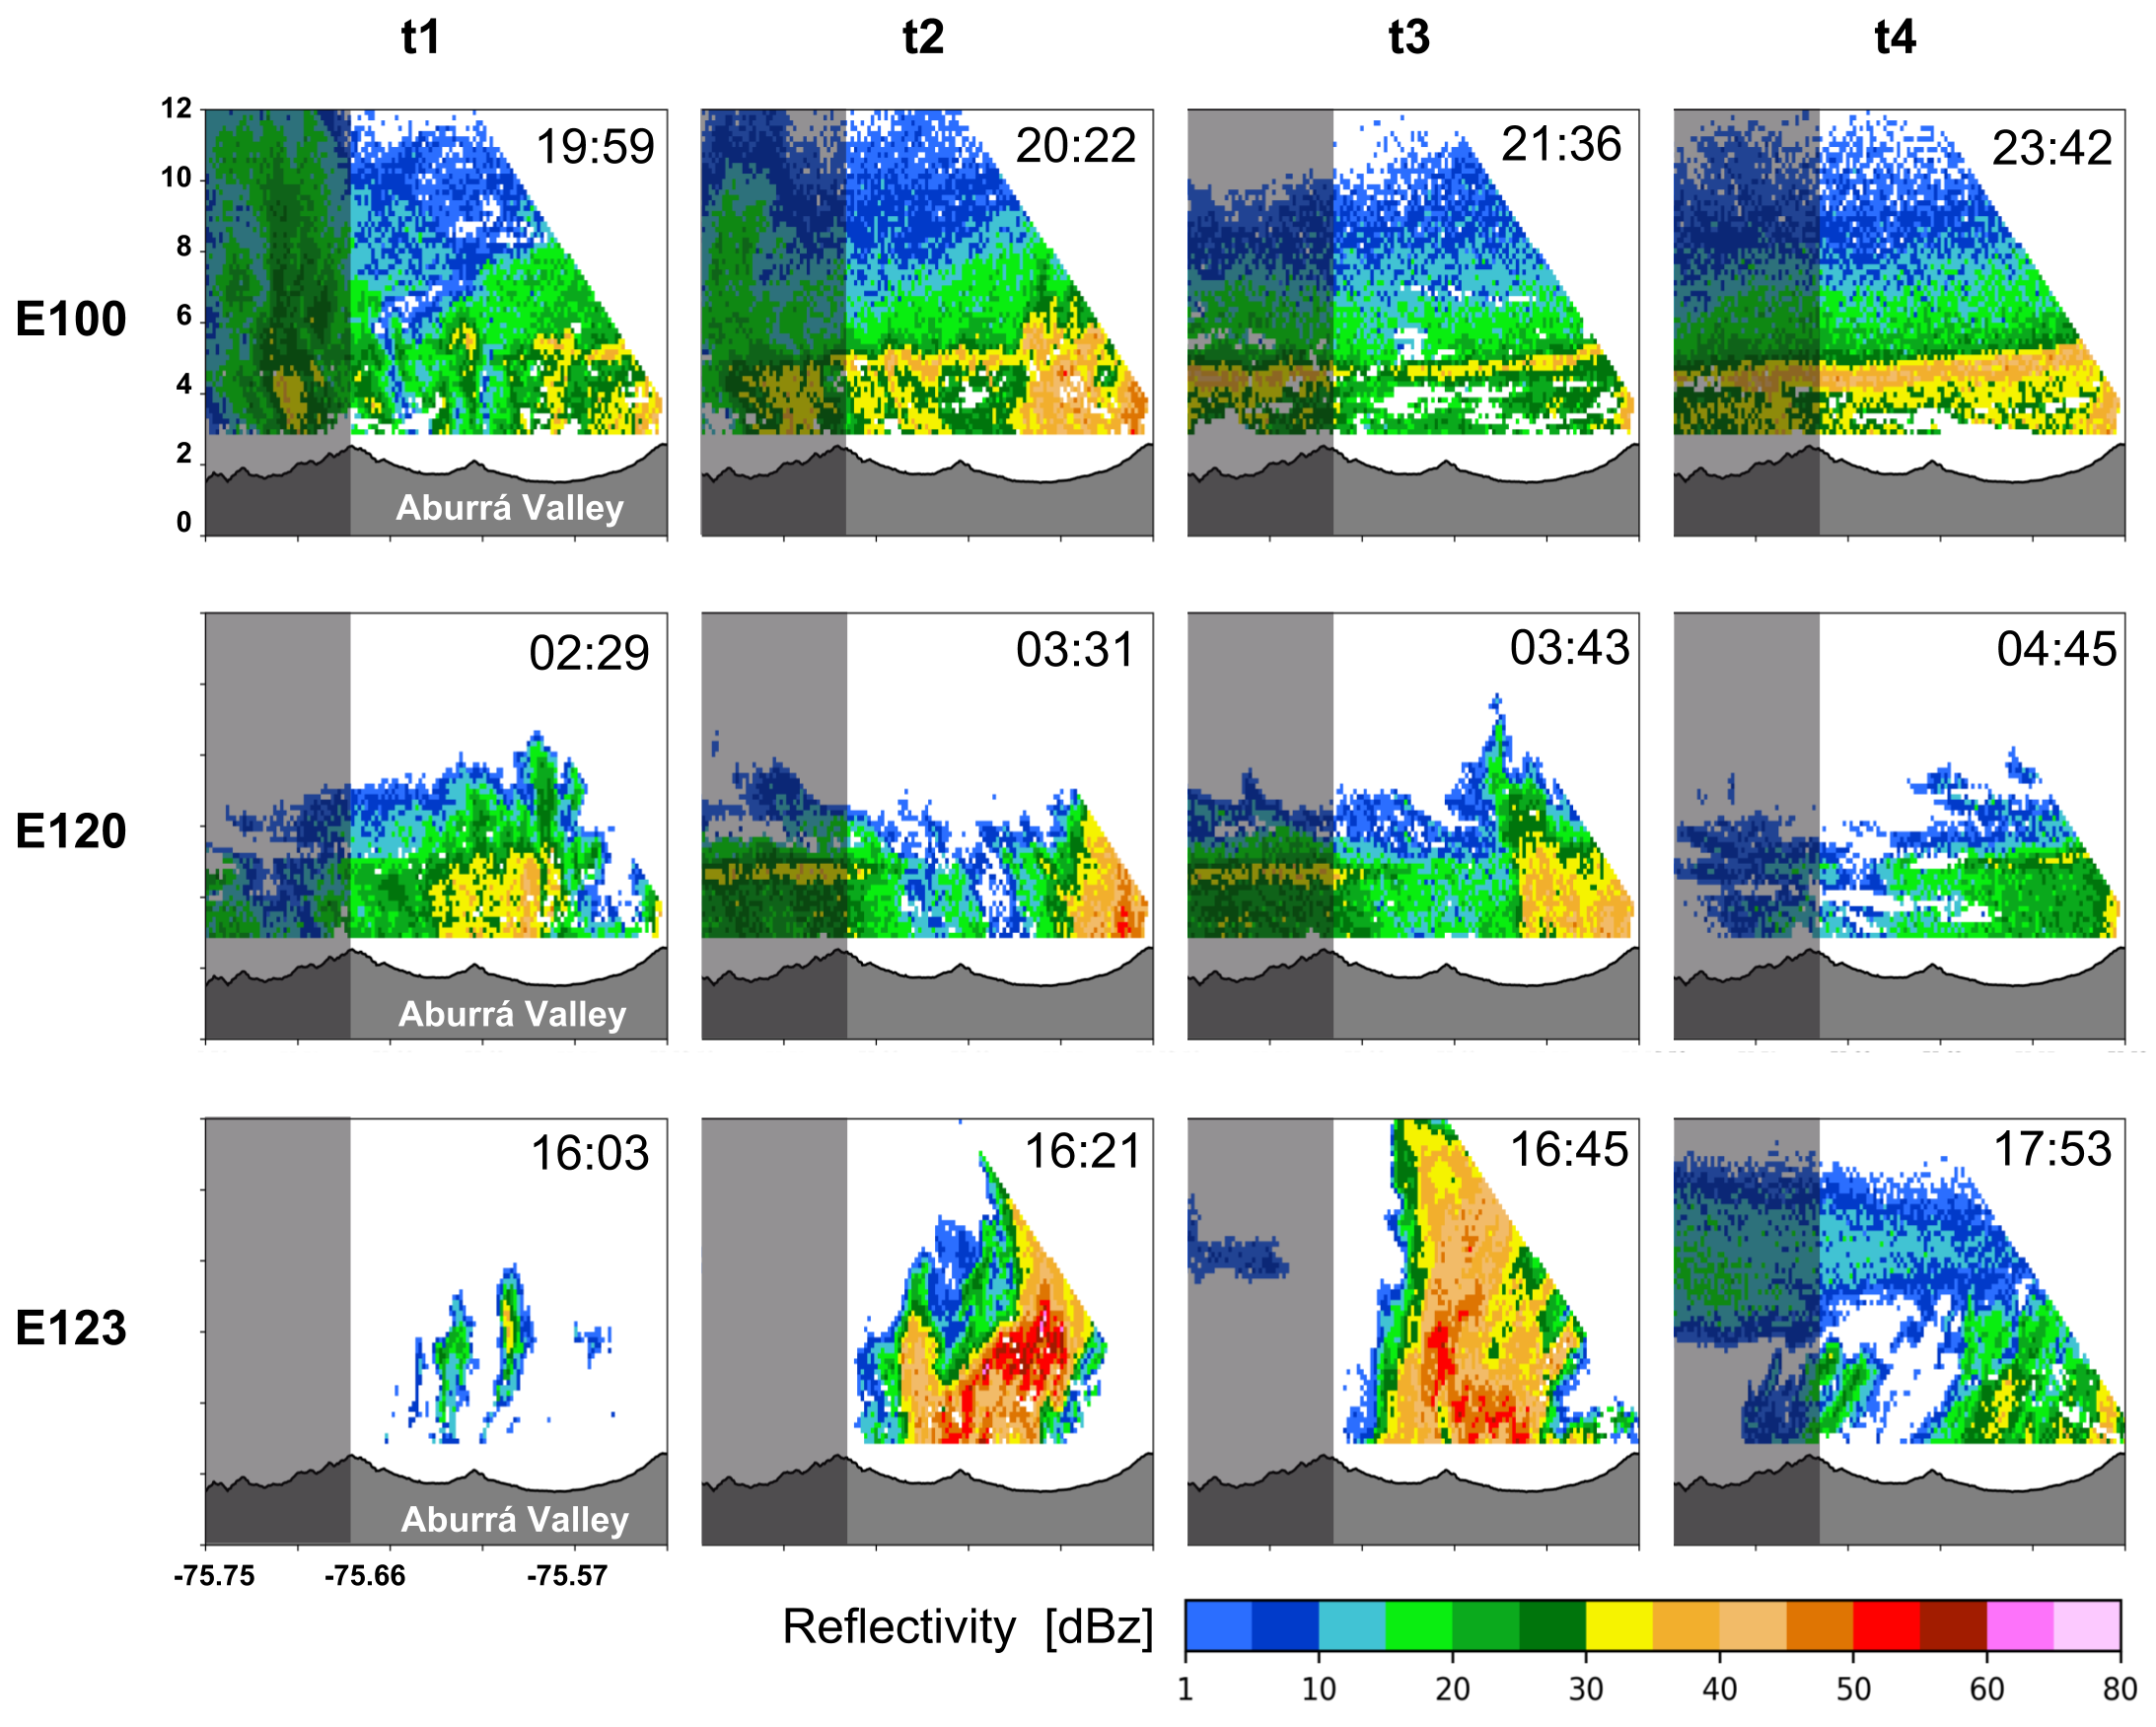
\includegraphics[width=14cm]{Figuras/Perfiles_Radar.png}
    \caption{Radar profiles of events E100, E120 and E123. Columns correspond to 
    different time steps of each event, the shaded area is outside of the watershed, the vertical profile is completely oriented from east to west.}
    \label{fig:radar_profiles}
\end{figure}

The above mentioned differences in the rainfall influence $Q_{obs}$, $Q_{run}$ and $Q_{sub}$.  In the four cases, peak streamflow and flow partitioning vary in function of the hietogram and the radar profiles of Figure  \ref{fig:radar_profiles} .  The value of $Q_{run}$ increases with the mean maximum intensity as shown on E123 (Figure \ref{fig:four_events}c), and $Q_{sub}$ increases with low-intensity and long-duration rainfall events as shown on  E100 and E186 (Figures \ref{fig:four_events}a and d respectively).  It is also important to notice how at events E100 and E120, $Q_{run}$ is related to the peaks of $Q_{sim}$, and tends to oscillate before $Q_{sub}$, which usually explains the recession. \\

At the four analyzed events,  $Q_{run}$ and $Q_{sub}$ vary with the observed radar profiles (Figure \ref{fig:radar_profiles}). With a duration of 4 hours and a high rainfall accumulation (Figure \ref{fig:rainfall_acum}a), event E100 has almost no convective formations and low values of $Q_{run}$. On the other hand, E120 exhibits less duration (about 3 hours) and a mix between small convective formations and stratiform development (Figure \ref{fig:radar_profiles}E120), in this case  $Q_{run}$ is similar to $Q_{sub}$.  Event E123 is the opposite scenario, with a high production of $Q_{run}$, the event has a high rainfall accumulation (Figure \ref{fig:rainfall_acum}c) and a well developed convective profile (Figure \ref{fig:radar_profiles}c). Finally, event E186 is a an extreme case of E100 in which $Q_{run}$ is zero. For this case, there is no convective formations, the mean intensity is low and the duration is high (around 5 hours). 

\begin{figure}[t]
    \centering
    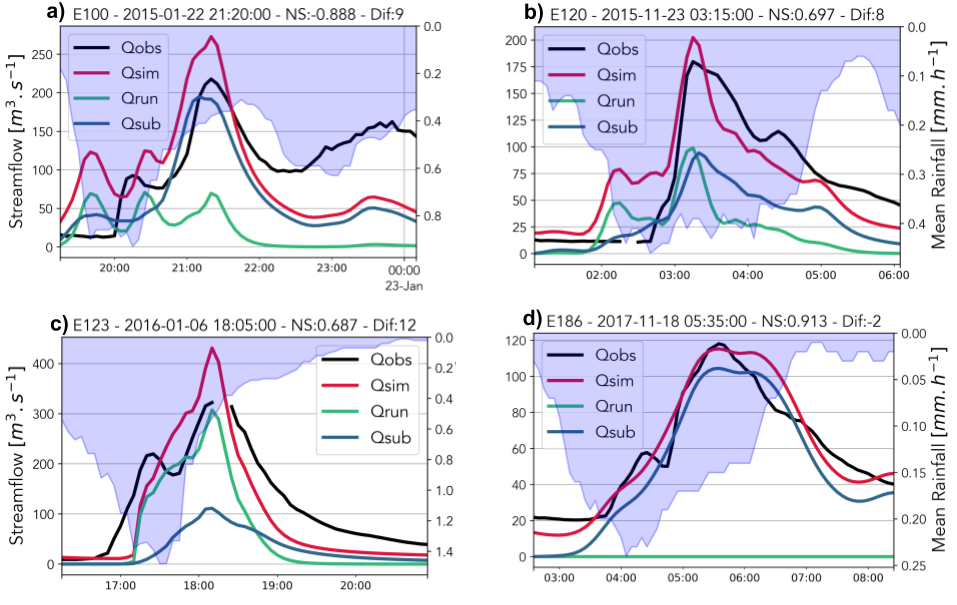
\includegraphics[width=14cm]{Figuras/Cuatro_eventos.png}
    \caption{Selected stormflow events, in each event we present the observed streamflow (black), total simulated streamflow (red), simulated surface runoff (green) and simulated subsurface runoff (blue), also we show rainfall depth in an inverted second y-axis. E100 and E120 are well mixed events between surface and subsurface. E123 is a surface runoff dominated event, and E186 is a subsurface dominated event.}
    \label{fig:four_events}
\end{figure}
At least in the four analyzed events, the spatiotemporal variability of the rainfall  plays a crucial role on the streamflow partitioning. The variability also includes the presence or absence of convective cells during the storm event.  With convective cells, the intensities are higher at a local scale and there is an increase of  $Q_{run}$ production, which is possibly explained by hortonian runoff processes.  On the other hand, without convective cells, intensities are low, and the runoff production is limited to soil saturation processes.  We need to do more work in this direction, however, our results suggest that the structure of the storm event could be crucial for understanding flow partitioning at watersheds with characteristics similar to the ones of the VA watershed. 

\subsection{Stormflow partitioning in function of rainfall and pre-event conditions.}

The results from the four analyzed cases show that rainfall influences streamflow partitioning, but due to the low number of cases, this result could be biased.   In order to obtain a more robust conclusion we use lumped rainfall and soil moisture features to perform a quantitative analysis of 128 events recorded between 2014 and 2017. The selected rainfall features are the mean maximum intensity ($I_{max}$) and the total rainfall ($P_{tot}$) of each event.  Regarding the soil moisture, we analyzed the time elapsed from the last storm ($T_e$) and the mid-term modeled gravitational storage ($H_g$).  Our results suggest that with some dispersion the evaluated variables play a significant role on the flow partitioning.\\   

Results show that the subsurface runoff ($S_{sub}$) and surface runoff ($S_{sur}$) increase with $P_{tot}$ and $I_{max}$ respectively (Figures \ref{fig:volumeVsRainfall}a and b respectively).  Increases of $P_{tot}$ represent a monotonical increase of $S_{sub}$ with a well defined interquartile dispersion, and at the same time $P_{tot}$ shows no relevant influence over the amount of $S_{sur}$ (see Figure \ref{fig:volumeVsRainfall}a).  On the other hand, $I_{max}$ has a positive correlation with $S_{sur}$, and a weak correlation with $S_{sub}$ (see Figure \ref{fig:volumeVsRainfall}b). The lack of a relationship between  $P_{tot}$ and $S_{sur}$ could be caused by an independence between $P_{tot}$ and $I_{max}$.   This independence can also help to explain the poor relation between $S_{sub}$ and $I_{max}$, as high values of $I_{max}$ increase hortonian surface runoff production, without necessarily implying increases at the soil moisture. 

The variability of Figures \ref{fig:volumeVsRainfall}a and b, show that the partitioning dynamics are not fully explained by the evaluated rainfall features.  At Figure \ref{fig:volumeVsRainfall}a there are cases with medium-high values of total rainfall and high $S_{sur}$ volume, behavior that could be explained by the described inter Independence among $P_{tot}$ and $I_{max}$.  A similar case is present at Figure \ref{fig:volumeVsRainfall}b were $S_{sub}$ have an increase variability and almost no dependence respect to $I_{max}$.\\

\begin{figure}[H]
    \centering
    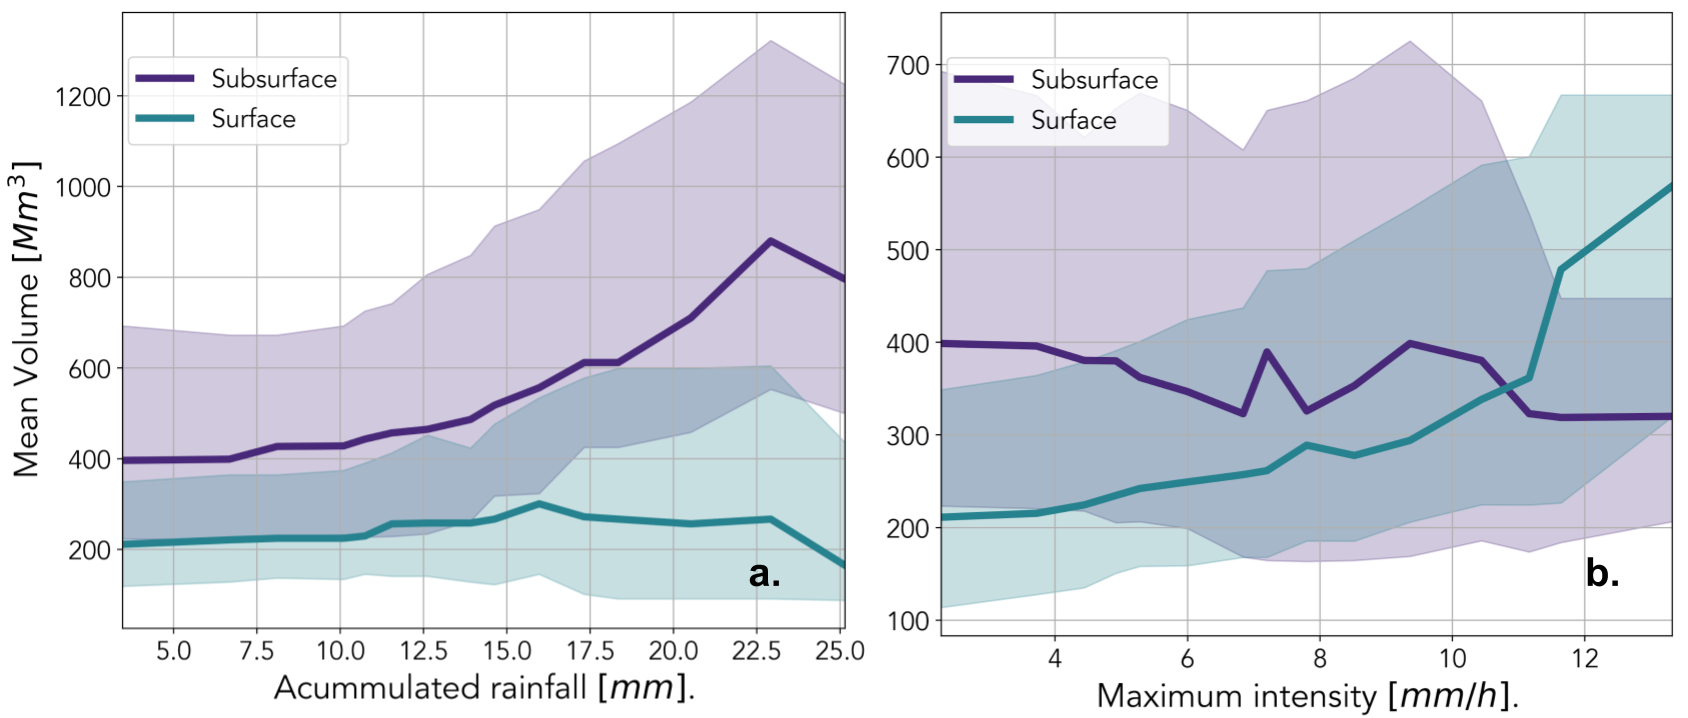
\includegraphics[width=14cm]{Figuras/MeanVolumeVsRainfall}
    \caption{Subsurface vs surface partitioned volume compared against a) the total rainfall of each event and b) the maximum mean intensity of each event.  The marked lines represent the percentile 50, shadows correspond to the percentile range of 25 - 75.}
    \label{fig:volumeVsRainfall}
\end{figure}
Pre-event conditions of the soils also play a role in the partitioning.  Figure \ref{fig:volumeVsSoil} presents the partitioned volume in function of $T_e$ and the $H_g$.  According to the results, at some cases, low values of $T_{e}$

$S_{sur}$ slightly increases with $T_e$, and with the decrease of the mean storage.  On the other hand, increases at the mean soil water storage imply weak decreases at the surface runoff and weak increases in the subsurface runoff.  The weak relation with the soil could be explained by the uncertainty of the used variable (mid-term model gravitational storage) and could be better assessed in the future by comparing with measured field data.\\

\begin{figure}[!h]
    \centering
    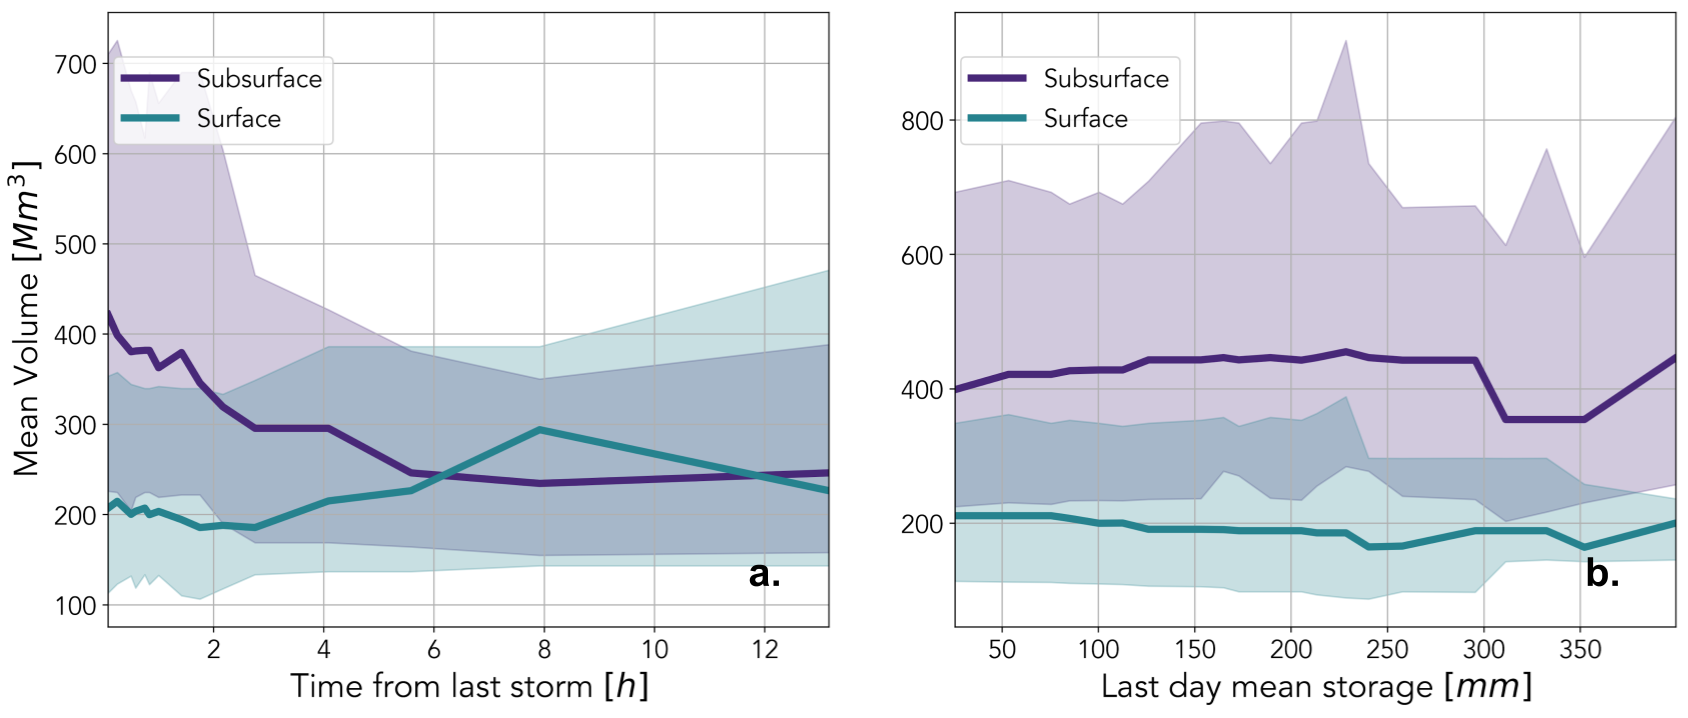
\includegraphics[width=14cm]{Figuras/MeanVolumeVsSoil}
    \caption{Subsurface vs surface partitioned volume compared against a) time from the last strom b) mean storage the day after the event.}
    \label{fig:volumeVsSoil}
\end{figure}
In Figure 7 we remark the differences that appear when there is a change of the independent variables (rainfall features or soil pre-event conditions).  According to Figure 7, streamflow partitioning behaves differently with respect to each variable.  Due to hortonian runoff production, maximum intensity increases surface volume and has a poor effect over the subsurface runoff evolution (Figure 7a).  On the other hand, total rainfall and subsurface increase simultaneously, with little effect over the surface runoff.\\

Figure 7c and d show the results for the streamflow partitioning compared to the mean soil storage the day before the event, and the elapsed time since the last storm event. Figure 7c shows that the increase in the mean storage has a poor effect over the flow partitioning. On the other hand, high values of subsurface runoff volume correspond to low values of elapsed time since the last storm.  Nevertheless, the elapsed time seems to have no effect over the surface runoff volume.\\

A general overview of our obtained results is shown at Figure 8 , which compares surface and subsurface runoff to maximum intensity by using colors to identify the mean storage of each event.  At Figure 8a we can see that low values of subsurface runoff correspond to high values of maximum intensity and elapsed time from last storm.  On the other hand, low intensity values increase subsurface runoff volume.

\begin{figure}[!h]
    \centering
    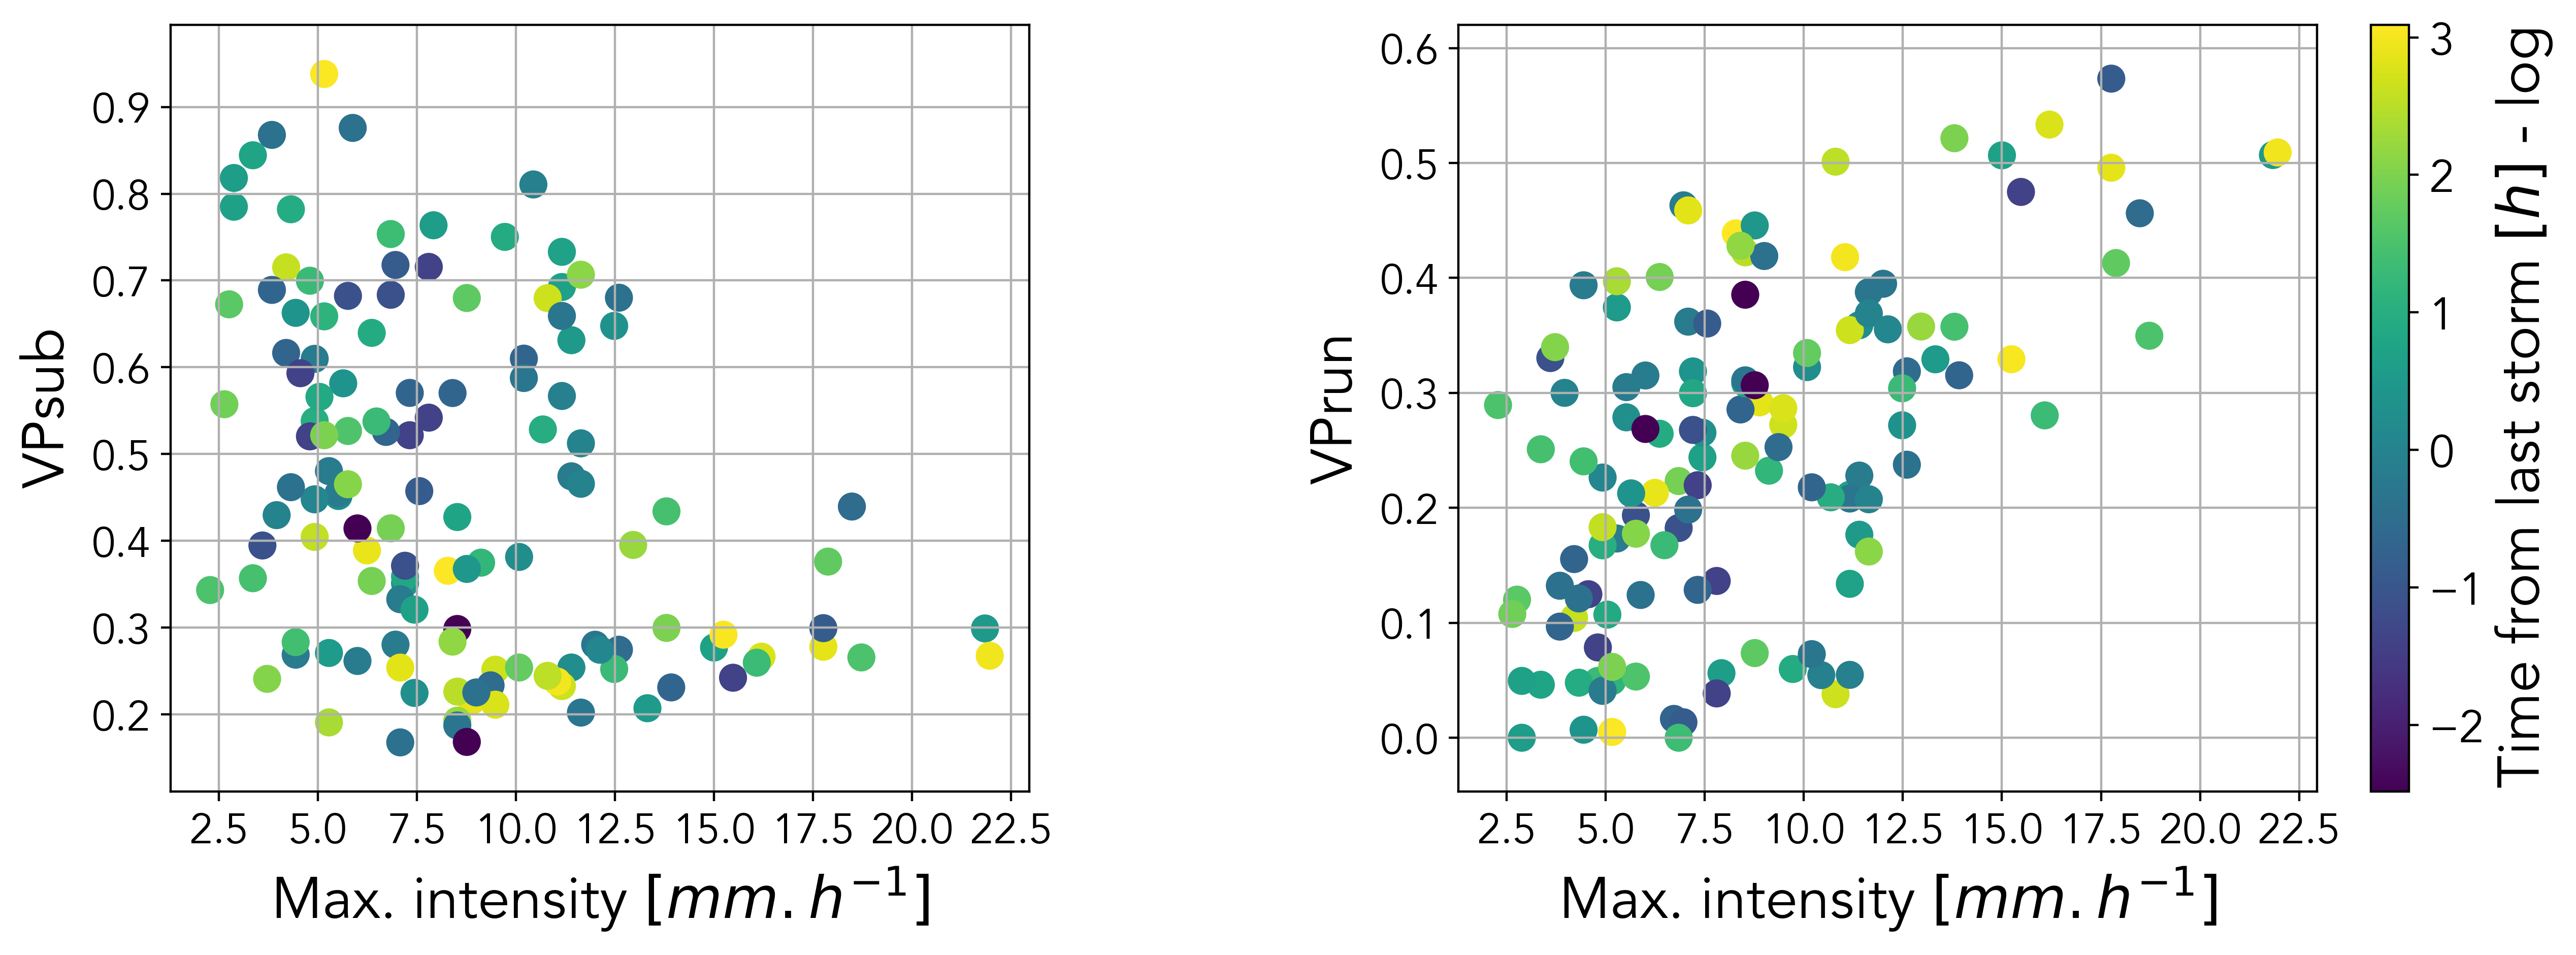
\includegraphics[width=14cm]{Figuras/Scatters_RainHFLS.png}
    \caption{Percentage of partitioned volume vs the mean maximum intensity. a) Surface runoff percentage, b) Subsurface runoff percentage. In both figures the colors correspond to the elapsed hours from the last storm.}
    \label{fig:VPvsIntensity}
\end{figure}

\section{Conclusions}

By doing a qualitative and quantitative analysis of the results from the hydrological model, we perform a conceptual evaluation of the surface and subsurface flow partitioning.  The qualitative analysis consists of the evaluation of four selected events (Figure \ref{fig:four_events}), in which we discuss the overall results with graphics of the hydrographs, and the spatiotemporal rainfall distribution.  On the other hand, in the quantitative analysis we include all the storm events recorded between 2012 and 2017.  For this case, we compare the results from the partitioning process with key features of the rainfall and the soil moisture of the watershed.  The results highlight an interdependence between flow partitioning and the examined rainfall and soil moisture features.\\

From the qualitative analysis of the four events we explore how the model partitioning is influenced by the rainfall spatiotemporal distribution.  In this analysis we presented a surface runoff dominated event, a subsurface runoff dominated event, and two well mixed events (with significant portions of surface and subsurface runoff).   Independent of the maximum intensity, the results show that the rainfall spatial accumulation  influences the model partitioning. The described results are shown at Figures \ref{fig:rainfall_acum}a and b, where high accumulations of rainfall at some regions of the watershed increase the production of surface runoff.  On the other hand, homogeneous rainfall fields with almost no regions of high accumulation, increase the subsurface runoff (Figures \ref{fig:four_events}d and \ref{fig:rainfall_acum}d) .  The results show the possibility of a significant relationship between the spatial structure of the rainfall and the flow partitioning. However, since the number of analyzed cases is limited, further research must me done in this direction.\\

In the quantitative analysis of 128 events, we compare the partitioning results with features of the rainfall and the soil moisture.  According to Figures \ref{fig:volumeVsRainfall}a and b, both the total rainfall and the maximum intensity have a significant influence over the model partitioning.  While the maximum intensity is directly related with the surface runoff, and indirectly related with the subsurface runoff.  The surface runoff is directly related with the maximum intensity and inversely related with the total rainfall. On the other hand, the subsurface runoff is inversely related with the mean maximum intensity and directly related with the total rainfall.  With a weaker relation, the   

the analyzed soil variables show a poor dependence with the flow partitioning. The elapsed time increases the surface runoff and decreases the subsurface runoff for values under 6 hours (Figure \ref{fig:volumeVsSoil}a). And the mean gravitational storage show a weak relation with the partitioning (Figure \ref{fig:volumeVsSoil}b) .   \\

We are aware that this work is based on modelling results with a lack of field validation, and our results and conclusions are limited to this specific case. However, this conceptual approximation with a physical model, and high resolution rainfall and streamflow data, let us explore the complex interactions among rainfall, soils and runoff production.\\ 


%\begin{table}[h]
%\centering
%\begin{tabular}{l l l}
%\hline
%\textbf{Treatments} & \textbf{Response 1} & \textbf{Response 2}\\
%\hline
%Treatment 1 & 0.0003262 & 0.562 \\
%Treatment 2 & 0.0015681 & 0.910 \\
%Treatment 3 & 0.0009271 & 0.296 \\
%\hline
%\end{tabular}
%\caption{Table caption}
%\end{table}

%% The Appendices part is started with the command \appendix;
%% appendix sections are then done as normal sections
%% \appendix

%% \section{}
%% \label{}

%% References
%%
%% Following citation commands can be used in the body text:
%% Usage of \cite is as follows:
%%   \cite{key}          ==>>  [#]
%%   \cite[chap. 2]{key} ==>>  [#, chap. 2]
%%   \citet{key}         ==>>  Author [#]

%% References with bibTeX database:

\bibliographystyle{humannat}
\bibliography{bibliography.bib}

%% Authors are advised to submit their bibtex database files. They are
%% requested to list a bibtex style file in the manuscript if they do
%% not want to use model1-num-names.bst.

%% References without bibTeX database:

% \begin{thebibliography}{00}

%% \bibitem must have the following form:
%%   \bibitem{key}...
%%

% \bibitem{}

% \end{thebibliography}


\end{document}

%%
%% End of file `elsarticle-template-1-num.tex'.